\documentclass[preprint,review,12pt]{elsarticle}
\usepackage[T1]{fontenc}
\usepackage{amsmath,amssymb,amsthm,booktabs,graphicx,placeins,float}
\usepackage{microtype}
\renewcommand{\floatpagefraction}{0.85}
\usepackage{xurl}
\usepackage[hidelinks]{hyperref}
\hypersetup{pdfauthor={Junyi Zhang},pdftitle={Retention-constrained class expansion with reference-anchored candidate tables}}
\pdfstringdefDisableCommands{\def\corref#1{}\def\cnotenum#1{}}
\newtheorem{proposition}{Proposition}
\newtheorem{corollary}{Corollary}
\newcommand{\RefBase}{86.03}
\newcommand{\RefBaseSD}{1.40}
\newcommand{\RefNovel}{66.90}
\newcommand{\RefNovelSD}{4.23}
\newcommand{\RefAll}{76.46}
\newcommand{\RefAllSD}{1.43}
\newcommand{\RefHarmonic}{75.19}
\newcommand{\RefHarmonicSD}{2.14}
\newcommand{\DynamicBase}{85.36}
\newcommand{\DynamicBaseSD}{0.66}
\newcommand{\DynamicNovel}{70.83}
\newcommand{\DynamicNovelSD}{4.33}
\newcommand{\DynamicAll}{78.09}
\newcommand{\DynamicAllSD}{2.02}
\newcommand{\DynamicHarmonic}{77.36}
\newcommand{\DynamicHarmonicSD}{2.48}
\newcommand{\SimpleBase}{82.47}
\newcommand{\SimpleBaseSD}{0.87}
\newcommand{\SimpleNovel}{77.53}
\newcommand{\SimpleNovelSD}{0.47}
\newcommand{\SimpleAll}{80.00}
\newcommand{\SimpleAllSD}{0.56}
\newcommand{\SimpleHarmonic}{79.92}
\newcommand{\SimpleHarmonicSD}{0.55}
\newcommand{\TextBase}{78.32}
\newcommand{\TextBaseSD}{0.25}
\newcommand{\TextNovel}{76.86}
\newcommand{\TextNovelSD}{1.97}
\newcommand{\TextAll}{77.59}
\newcommand{\TextAllSD}{0.86}
\newcommand{\TextHarmonic}{77.57}
\newcommand{\TextHarmonicSD}{0.88}
\newcommand{\RefErrorFlip}{1.84}
\newcommand{\RefErrorFlipSD}{1.54}
\newcommand{\RefChurn}{3.63}
\newcommand{\RefChurnSD}{2.40}
\newcommand{\LatencyFifty}{1.76}
\newcommand{\LatencySixty}{0.75}
\newcommand{\LatencyEighty}{0.78}
\newcommand{\PetRefBase}{97.18}
\newcommand{\PetRefBaseSD}{2.25}
\newcommand{\PetRefNovel}{87.79}
\newcommand{\PetRefNovelSD}{6.18}
\newcommand{\PetRefAll}{92.49}
\newcommand{\PetRefAllSD}{2.83}
\newcommand{\PetRefHarmonic}{92.14}
\newcommand{\PetRefHarmonicSD}{3.23}
\newcommand{\PetDynamicBase}{96.85}
\newcommand{\PetDynamicBaseSD}{1.50}
\newcommand{\PetDynamicNovel}{86.49}
\newcommand{\PetDynamicNovelSD}{7.64}
\newcommand{\PetDynamicAll}{91.67}
\newcommand{\PetDynamicAllSD}{4.56}
\newcommand{\PetDynamicHarmonic}{91.29}
\newcommand{\PetDynamicHarmonicSD}{4.99}
\newcommand{\PetSimpleBase}{94.77}
\newcommand{\PetSimpleBaseSD}{2.91}
\newcommand{\PetSimpleNovel}{93.91}
\newcommand{\PetSimpleNovelSD}{1.55}
\newcommand{\PetSimpleAll}{94.34}
\newcommand{\PetSimpleAllSD}{1.43}
\newcommand{\PetSimpleHarmonic}{94.31}
\newcommand{\PetSimpleHarmonicSD}{1.44}
\newcommand{\PetTextBase}{92.87}
\newcommand{\PetTextBaseSD}{3.37}
\newcommand{\PetTextNovel}{94.05}
\newcommand{\PetTextNovelSD}{1.35}
\newcommand{\PetTextAll}{93.46}
\newcommand{\PetTextAllSD}{1.59}
\newcommand{\PetTextHarmonic}{93.43}
\newcommand{\PetTextHarmonicSD}{1.63}

\newcommand{\CFMatchedBase}{83.48}
\newcommand{\CFMatchedNovel}{75.79}
\newcommand{\CFTunedNovel}{61.36}
\newcommand{\CFDenseNovel}{74.43}
\newcommand{\CFMatchedGain}{14.43}
\newcommand{\CFDenseGain}{1.37}
\newcommand{\PetStrictBase}{96.84}
\newcommand{\PetStrictNovel}{90.99}
\newcommand{\PetStrictDenseNovel}{84.00}
\newcommand{\PetStrictGain}{7.00}
\newcommand{\CFMatchedGainSD}{6.59}
\newcommand{\CFDenseGainSD}{3.37}
\newcommand{\PetStrictGainSD}{5.57}
\newcommand{\CFTunedAverageGain}{2.18}
\newcommand{\CFTunedAverageGainSD}{0.24}
\newcommand{\CFTunedFinalGain}{1.75}
\newcommand{\CFTunedFinalGainSD}{0.23}
\newcommand{\CFDenseAverageGain}{0.46}
\newcommand{\CFDenseAverageGainSD}{0.44}
\newcommand{\CFDenseFinalGain}{0.02}
\newcommand{\CFDenseFinalGainSD}{0.56}
\newcommand{\CFRemovedAverageGain}{10.62}
\newcommand{\CFRemovedAverageGainSD}{15.22}
\newcommand{\CFRemovedFinalGain}{11.28}
\newcommand{\CFRemovedFinalGainSD}{16.33}
\newcommand{\PetTunedAverageGain}{-0.11}
\newcommand{\PetTunedAverageGainSD}{0.56}
\newcommand{\PetTunedFinalGain}{-0.80}
\newcommand{\PetTunedFinalGainSD}{0.85}
\newcommand{\PetDenseAverageGain}{-0.26}
\newcommand{\PetDenseAverageGainSD}{1.82}
\newcommand{\PetDenseFinalGain}{-0.72}
\newcommand{\PetDenseFinalGainSD}{2.65}
\newcommand{\PetRemovedAverageGain}{16.92}
\newcommand{\PetRemovedAverageGainSD}{28.33}
\newcommand{\PetRemovedFinalGain}{14.92}
\newcommand{\PetRemovedFinalGainSD}{26.40}

\journal{Knowledge-Based Systems}
\begin{document}
\begin{frontmatter}
\title{Retention-constrained class expansion with reference-anchored candidate tables}
\author[sdu]{Junyi Zhang\corref{cor1}}
\ead{cheerssom0876@gmail.com}
\cortext[cor1]{Corresponding author.}
\affiliation[sdu]{organization={Shandong University},country={China}}
\begin{abstract}
Class expansion must recognize arriving classes while meeting an original-class accuracy requirement. Reference-anchored candidate tables retain a trained classifier, align semantic and prototype evidence against fixed base references, and separately calibrate novel admission. Across three source benchmarks and five arrivals with frozen CLIP ViT-L/14 and ViT-B/32, equal-budget fusion tuning isolates query-dependent normalization. On ImageNet-R, it adds 3.60 and 5.29 percentage points of final-arrival novel capacity over uncentered fusion at a shared 95\% retention target. On 6,445 deduplicated ImageNet-Sketch images, frozen source models achieve 86.82\% and 58.96\% novel accuracy with direct target calibration and empirical target attainment in all ten partitions per encoder.
\end{abstract}
\begin{keyword}
Class expansion \sep Retention constraints \sep Incremental learning \sep Evidence fusion \sep Vision--language models \sep Long-tailed recognition
\end{keyword}
\end{frontmatter}

\section{Introduction}
An expanding recognition system already has a classifier whose decision boundaries reflect task-specific supervision. New classes arrive with names and a few examples. The central question is how much new-class recognition that existing discrimination can support while maintaining a specified accuracy on the original classes. A second question follows across repeated arrivals: how much predictive value is gained by keeping the trained classifier rather than replacing it with prototypes or recalibrated semantic evidence?

We address these questions with \emph{reference-anchored candidate tables}. The table retains learned base columns and appends semantic anchors and support prototypes for arriving classes. Each evidence branch is normalized against fixed base references, so adding candidates leaves existing scores unchanged. An independent admission offset controls competition between base and novel classes. This separates the discrimination already learned from the decision to admit new alternatives.

We connect retained discrimination to retention-constrained class expansion: a persistent score frame makes the original classifier reusable, a common base-accuracy constraint makes its admission value comparable, and paired arrival sequences measure its continuing benefit. Independent calibration tests the shared accuracy requirement through either a sufficient protection loss or a direct paired accuracy test that credits recovered errors. The design contribution is a vocabulary-independent score frame for heterogeneous readouts, coupled to an independently calibrated admission rule. Fixed references preserve stored evidence; query moments align branch responses; the admission offset selects a retention-constrained operating point. Controlled normalization experiments test the second role separately from score persistence and threshold selection. On ImageNet-R, the gain over dense prototypes persists across two frozen encoders. Independent calibration certifies final-session expansion on all source partitions; a deduplicated Sketch evaluation tests frozen-model admission under natural distribution shift.

\section{Related work}
Long-tailed recognition addresses unequal class supervision through balanced fitting and losses~\cite{liu2019large,cao2019ldam,cui2019classbalanced}. CLIP supplies semantic image--text evidence~\cite{radford2021clip}, while prompt adaptation~\cite{zhou2022coop,shi2024lift}, prototypes~\cite{snell2017prototypical,wang2019simpleshot} and semantic caches~\cite{zhang2022tipadapter} adapt pre-trained representations to labeled data. Our setting combines these evidence types according to their availability at class arrival.

Class-incremental and few-shot incremental learning study retention across successive tasks~\cite{rebuffi2017icarl,tao2020fewshot}. SimpleCIL~\cite{zhou2024simplecil} and RanPAC~\cite{mcdonnell2023ranpac} show the value of pre-trained prototypes and analytic readouts. KBS approaches develop multi-feature similarity supplementation~\cite{xu2023mfs3}, sharpness-aware prototype calibration~\cite{chen2024sagg}, adaptive exploration~\cite{han2025adaptive}, representation-enhanced analytic learning~\cite{he2026real}, and multimodal prompt fusion~\cite{fang2026bpcclip}.

Recent work aligns task-specific expert inference in MoTE~\cite{li2025mote}, separates expanding feature spaces through orthogonal constraints~\cite{dong2026deon}, and learns invariant representations through counterfactual distribution intervention~\cite{yuan2026cdi}. Our contribution concerns the admission capacity supplied by an existing classifier under a common base-accuracy requirement. CLIP-guided discovery~\cite{yan2025clipdiscovery} additionally uses unlabeled novel data, whereas our arriving classes provide names and labeled support. FeNeC~\cite{ksiazek2026fenec} supplies a clustered-representative readout for controlled frozen-feature comparisons.

BiMC~\cite{chen2025bimc} and HyCal~\cite{lee2026hycal} calibrate multimodal or heterogeneous recognition metrics. Calibrated seen/unseen recognition~\cite{chao2016calibrated} studies the related operating trade-off, and Learn then Test~\cite{angelopoulos2021ltt} supplies risk-controlled threshold selection. We focus on the retained classifier as a source of admission capacity: its contribution is measured at a common base requirement, over successive arrivals, and under separately calibrated protection and direct accuracy policies. The comparison includes an author-code-checked HyCal transfer with matched encoders, labels and support. Calibrated offsets select a global operating point; our query-dependent branch moments also change evidence comparability before that selection. Fixed-reference normalization makes this alignment independent of the arriving vocabulary. The statistical tests follow established risk-control principles; the contribution lies in applying a shared accuracy target to persistent and replacement readouts and separating their recognition frontiers from calibrated policies.

\section{From retained discrimination to novel admission}
\subsection{Task and evidence}
Base classes $\mathcal B$ have labeled, potentially imbalanced fitting data. Arriving classes $\mathcal N$ provide a name and $k$ labeled support images per class. Prediction selects from $\mathcal B\cup\mathcal N$ without a group oracle. A frozen encoder produces a normalized feature $v=f(x)$; normalized text anchors $t_c$ average eight fixed prompts. Learned base scores are $q_L(x,b)=v^\top w_b+b_b$, fitted by inverse-frequency-weighted ridge regression. Novel prototypes are normalized support means $p_n$, giving $q_P(x,n)=v^\top p_n$; semantic scores are $q_T(x,c)=v^\top t_c$.

\begin{figure}[!htbp]
\centering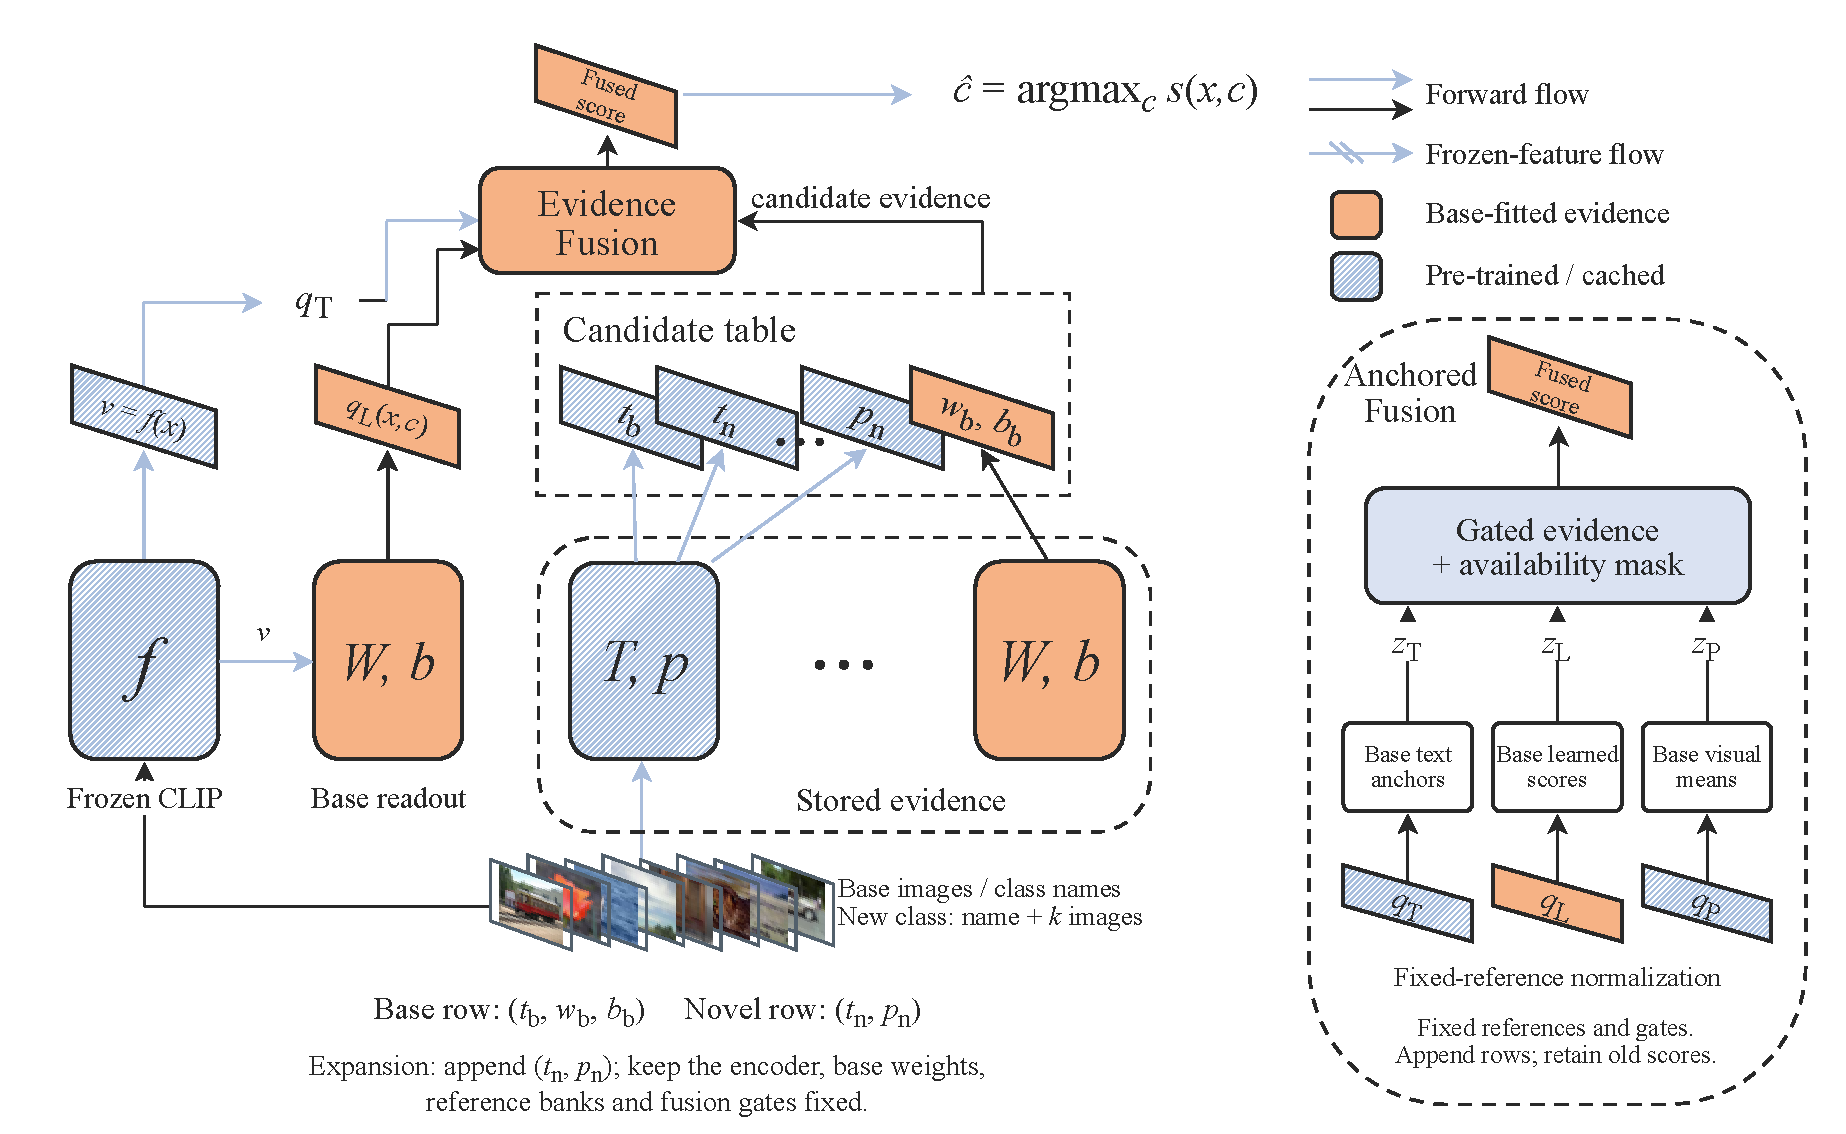
\includegraphics[width=.98\textwidth]{framework.pdf}
\caption{Reference-anchored candidate tables. Fixed base references set each branch's score frame; learned base columns remain stored as novel text anchors and support prototypes are appended. The separate novel offset controls admission. Orange marks base-fitted evidence; blue hatching marks pre-trained or cached evidence.}
\label{fig:framework}
\end{figure}

For each evidence source $e$, a fixed base reference bank $\mathcal R_e$ defines
\begin{align}
 \mu_e(x)&=|\mathcal R_e|^{-1}\sum_{b\in\mathcal R_e}q_e(x,b),\\
 \sigma_e^2(x)&=|\mathcal R_e|^{-1}\sum_{b\in\mathcal R_e}(q_e(x,b)-\mu_e(x))^2.
 \label{eq:reference}
\end{align}
We use base text anchors, learned columns and visual means as the text, learned and prototype references. Normalized evidence is
\begin{equation}
 \widehat q_e(x,c)=\frac{q_e(x,c)-\mu_e(x)}{\max(\sigma_e(x),10^{-6})}.
 \label{eq:anchored}
\end{equation}
The statistics adapt to each query while remaining independent of the active novel vocabulary. Fusion uses the evidence available to each row:
\begin{align}
 s(x,b)&=\widehat q_T(x,b)+a\widehat q_L(x,b),&&b\in\mathcal B,\\
 s(x,n)&=\widehat q_T(x,n)+u\widehat q_P(x,n)+d,&&n\in\mathcal N.
 \label{eq:base-novel}
\end{align}
The coefficients $a,u$ combine evidence; $d$ controls novel admission (Fig.~\ref{fig:framework}). Candidate-wise normalization instead changes the branch scales when new rows arrive, which can alter existing fused decisions. A numerical example appears in Supplementary Section K.

\begin{proposition}
With fixed input, encoder, existing row evidence, reference banks, coefficients and tie-breaking, appending rows preserves every existing score and its within-vocabulary ordering.
\label{prop:invariance}
\end{proposition}
All terms of an existing row remain fixed. This structural property also holds for raw and fixed-temperature controls; their recognition comparisons isolate reference normalization. Appended rows can still win the expanded prediction. Supplementary Section E gives the proof and prediction consequence. Each new row costs $O(D)$ storage and $O(kD)$ prototype construction after encoding; scoring $K$ classes costs $O(KD)$.

\subsection{Calibration and expansion capacity}
\label{sec:calibration}
A base-only pseudo-expansion episode splits base classes into pseudo-base and pseudo-novel groups. A classifier fitted on pseudo-base classes is combined with names and reserved support for pseudo-novel classes. Held-out base queries select $a,u,d$ by harmonic macro accuracy,
\begin{equation}
 H=2A_BA_N/(A_B+A_N),
 \label{eq:harmonic}
\end{equation}
with zero assigned when both accuracies vanish. The coefficients then remain fixed across actual arrivals. Actual novel query labels and test labels are excluded from this selection; grids and split seeds are in Supplementary Section K.

Let $A_{B,\mathrm{ref}}^{\mathrm{closed}}$ denote the retained table's closed-base macro accuracy. At retention fraction $r$, every readout receives the same absolute base target. Thus a 90\% reference gives an 85.5\% absolute target at 95\% retention. Its empirical expansion capacity is
\begin{equation}
 N_r=\max_d A_N(d)\quad\text{subject to}\quad
 A_B(d)\geq rA_{B,\mathrm{ref}}^{\mathrm{closed}}.
 \label{eq:retentioncriterion}
\end{equation}
A test-label sweep characterizes this descriptive frontier; an operational threshold uses calibration data. The exact margin envelope is derived in Supplementary Section D. Reporting these two evaluations separately distinguishes attainable capacity from selected-policy behavior.

\subsection{Independent accuracy calibration}
\label{sec:riskcontrol}
Let $R$ indicate correct prediction by the retained closed-base reference and $C_d$ correct prediction by the expanded readout. Define
\begin{equation}
 L_d=R(1-C_d)+(1-r)(1-R).
 \label{eq:protectionloss}
\end{equation}
Writing $D=\Pr(R=1,C_d=0)$ gives $\mathbb E L_d=D+(1-r)(1-A_{B,\mathrm{ref}})$. Thus $\mathbb E L_d\leq1-r$ implies $A_B(d)\geq rA_{B,\mathrm{ref}}$. This common sufficient criterion conservatively ignores replacement readouts' recovery of reference errors.

Fitting and tuning data fix the score models and ordered candidate thresholds. Independent, class-stratified calibration observations test thresholds from conservative to permissive using weighted bounded-loss p-values and fixed-sequence testing~\cite{angelopoulos2021ltt}. Testing stops at the first failure. Allocating error probability $\delta/5$ per arrival controls population protection across five prespecified sessions for each method, order and partition under independent class-conditional sampling. It does not guarantee arbitrary distribution shifts or every finite test outcome. If no finite threshold passes, the policy returns the reference classifier with zero novel admission. Supplementary Section J provides the bound, assumptions and full selection rule.

A second procedure tests the accuracy requirement directly. For independent calibration pairs, set $Z_i=C_{d,i}-rR_i$, macro weights $w_i=1/(B n_{c(i)})$, and $b=\max_iw_i$. The nonnegative product
\begin{equation}
 E_\lambda=\prod_i[1+\lambda(w_i/b)Z_i],\qquad 0\leq\lambda<1/r,
 \label{eq:directbet}
\end{equation}
has expectation at most one under $\sum_iw_i\mathbb E Z_i\leq0$. A fixed equal mixture over twelve prespecified values of $\lambda$ yields a valid p-value $\min(1,1/E)$ by Markov's inequality. This fixed-sample betting construction~\cite{waudby2024betting} credits corrected reference errors and uses the same ordered candidates and five-session error allocation. Supplementary Section N gives the self-contained proof. Calibration images are held out from fitting and tuning; stochastic independence and correspondence to the target class-conditional laws are additional assumptions. The 95\% statement applies separately to the five prespecified arrivals of each fixed method/order/partition/policy, rather than jointly to the full experimental grid.

\section{Experiments}
\subsection{Protocol and comparisons}
\label{sec:tenpartitions}
We evaluate CIFAR-100~\cite{krizhevsky2009cifar}, Oxford-IIIT Pets~\cite{parkhi2012cats} and ImageNet-R~\cite{hendrycks2021manyfaces}, using frozen OpenAI CLIP ViT-L/14 and ViT-B/32 features, five-shot support, ten frequency-stratified class partitions and two five-session arrival orders. Base/novel counts are 40/40, 15/15 and 100/100; each session adds eight, three or 20 classes. Base pools follow long-tailed sampling. ImageNet-R uses task-specific splits after removing byte-identical duplicates. Novelty is relative to task fitting, with CLIP's pre-training exposure retained. Detailed pools, preprocessing and seeds are in Supplementary Sections C, I and K.

Every comparator shares its encoder, partition and support. We compare fixed-gate classifier removal, independently recalibrated removal, dense anchored text--prototype fusion, summed/class-mean Tip-Adapter caches, and raw/fixed-temperature retained fusion. The latter uses a single base-validation scale per branch. HyCal uses the author's heterogeneous cosine/Mahalanobis metrics, count weighting and Gaussian-CDF calibration, transferred to the same eight-prompt anchors and frozen encoders. Its covariance regularization and novel offset are selected by base-only pseudo-expansion. Supplementary Section M documents the pinned implementation, numerical fixtures and transfer settings. All mixtures use base-only selection; FeNeC and earlier three-partition auxiliary studies are retained in Supplementary Sections A--H.

Orders are averaged within a partition. Means and standard deviations describe ten class assignments on fixed images. Paired differences use identical cells; constrained comparisons use jointly feasible sets. Conditional paired 95\% bootstrap intervals resample partition means 20,000 times. Average incremental accuracy is the mean macro accuracy over five arrivals. These intervals characterize class-assignment variation, conditional on the fixed data and encoders.

\subsection{Novel recognition at a shared base requirement}
At the descriptive 95\% retention budget, the ImageNet-R L/14 table reaches 84.31\% novel accuracy at 86.42\% base accuracy. Figure~\ref{fig:capacity} compares novel recognition under shared base requirements across encoders and datasets. A more discriminative base readout can tolerate greater novel competition while meeting the same target, turning retained discrimination into admission capacity.

\begin{figure}[!htbp]
\centering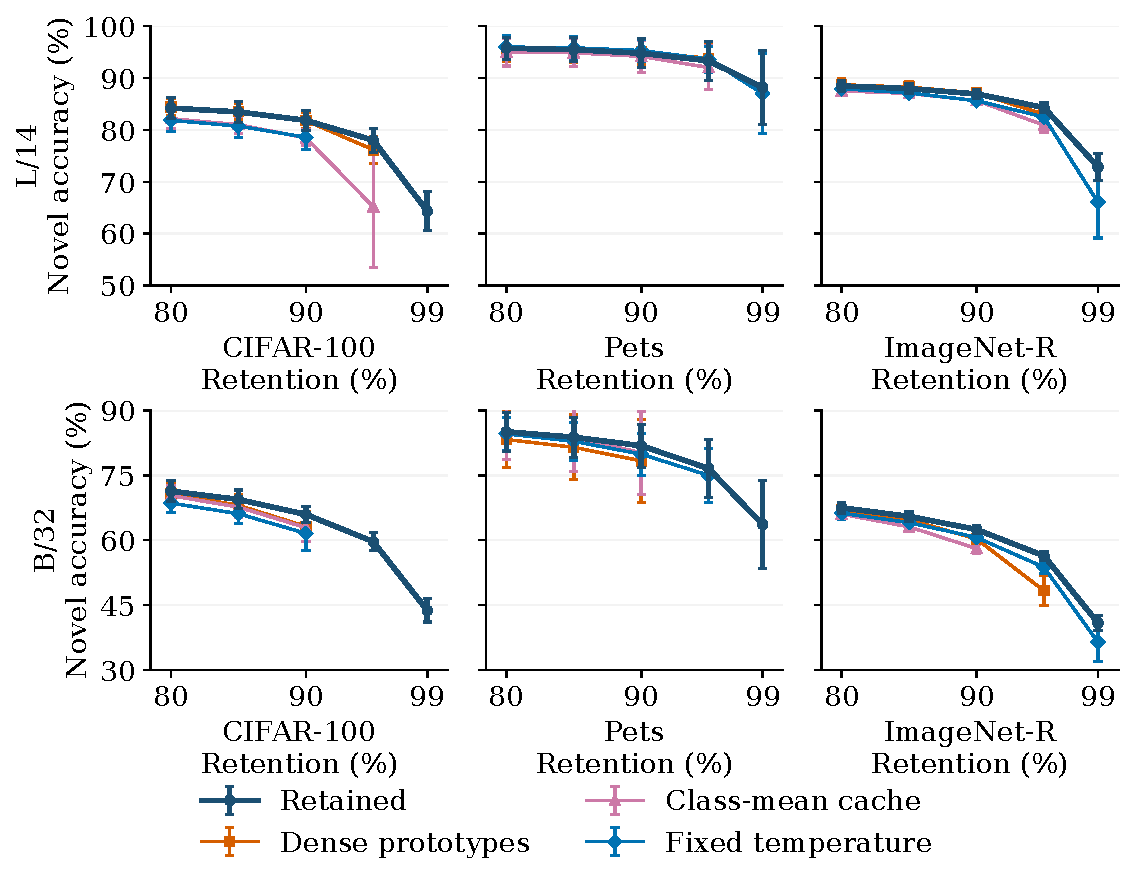
\includegraphics[width=.98\textwidth]{matched_capacity_main.pdf}
\caption{Novel recognition at shared base-retention requirements after the fifth arrival. Each readout must attain the stated fraction of the retained reference's closed-base accuracy within the same partition and encoder. Means and sample standard deviations cover ten partitions after averaging two arrival orders; points require all ten partitions to be feasible. Vertical ranges are 50--100\% (L/14) and 30--90\% (B/32); error bars stop at panel limits. Test-label threshold sweeps characterize descriptive capacity. Partial feasible sets and exact counts are reported in Supplementary Section I.}
\label{fig:capacity}
\end{figure}

\subsection{Isolating query-dependent normalization}
The factorial in Supplementary Section M changes centering and scaling independently while fixing the reference banks, learned models, support and original fusion coefficients and offsets. Fixed moments are estimated from base-tuning queries. On ImageNet-R, query-dependent scaling adds 0.43 [0.17,0.65] and 0.36 [0.15,0.58] points with L/14 and B/32 when query centering is retained. Query centering adds a further 2.03 [1.37,2.68] and 0.88 [0.39,1.55] points at query-dependent scale. These fixed-gate contrasts measure the contribution within the selected fusion model. An equal-budget study independently reselects both fusion coefficients and the tuning offset for each normalization scheme, using the same 3,636 base-only pseudo-expansion settings. At the common 95\% base target, query normalization exceeds no centering by 3.60 [2.55,4.74] points on ImageNet-R L/14 and 5.29 [3.74,7.25] on B/32; gains over fixed global normalization are 2.84 [2.42,3.28] and 4.65 [3.57,5.71] points. All contrasts use ten jointly feasible partitions after averaging orders. With independently selected fusion weights for both readouts, retained-minus-dense capacity differs by 0.25 [$-0.46$,0.92] points on L/14 and 9.69 [8.08,11.21] on B/32. Section Q reports all conditions, search settings and independently calibrated policies; the offset-only control is in Section P.



\subsection{The classifier's value across arrivals}
Table~\ref{tab:paired} quantifies retained-minus-comparator average incremental accuracy with fixed base-only selected gates and offsets. On ImageNet-R, retaining the classifier adds 0.71 [0.46, 0.92] points over dense prototypes with L/14 and 0.90 [0.69, 1.11] with B/32. Corresponding gains over class-mean caches are 1.42 [1.15, 1.62] and 1.71 [1.44, 1.98] points. The result persists across both encoders and after calibration is restored to the classifier-free alternative.

\clearpage
\begin{table}[H]
\centering
\setlength{\belowcaptionskip}{8pt}
\caption{The retained classifier's value across five arrivals. Cells show paired gains in average incremental accuracy (percentage points), with conditional paired 95\% bootstrap intervals below. Positive values favor retention; bold estimates have intervals excluding zero. Two orders are averaged within each of ten partitions. Full final-session differences are in Supplementary Section I.}
\label{tab:paired}
{\small\setlength{\tabcolsep}{5pt}\renewcommand{\arraystretch}{1.15}\begin{tabular}{@{}lrrr@{}}
\toprule
Comparator & \multicolumn{3}{c}{Retained-minus-comparator gain (pp) $\uparrow$} \\
\cmidrule(l){2-4}
& CIFAR-100 & Pets & ImageNet-R \\
\midrule
\multicolumn{4}{@{}l}{\textnormal{CLIP ViT-L/14}} \\
Recalibrated removal & \shortstack[r]{\textbf{+3.00}\\{\scriptsize [+2.23, +3.75]}} & \shortstack[r]{-0.14\\{\scriptsize [-1.53, +0.86]}} & \shortstack[r]{\textbf{+2.30}\\{\scriptsize [+1.95, +2.59]}} \\
Dense prototypes & \shortstack[r]{+0.15\\{\scriptsize [-0.46, +0.64]}} & \shortstack[r]{-0.98\\{\scriptsize [-2.52, +0.22]}} & \shortstack[r]{\textbf{+0.71}\\{\scriptsize [+0.46, +0.92]}} \\
Class-mean cache & \shortstack[r]{\textbf{+1.44}\\{\scriptsize [+0.68, +2.10]}} & \shortstack[r]{-0.06\\{\scriptsize [-1.76, +1.41]}} & \shortstack[r]{\textbf{+1.42}\\{\scriptsize [+1.15, +1.62]}} \\
\midrule
\multicolumn{4}{@{}l}{\textnormal{CLIP ViT-B/32}} \\
Recalibrated removal & \shortstack[r]{\textbf{+2.38}\\{\scriptsize [+1.44, +3.34]}} & \shortstack[r]{-0.44\\{\scriptsize [-1.64, +0.81]}} & \shortstack[r]{\textbf{+3.07}\\{\scriptsize [+2.82, +3.34]}} \\
Dense prototypes & \shortstack[r]{+0.86\\{\scriptsize [-0.15, +1.76]}} & \shortstack[r]{-0.39\\{\scriptsize [-1.85, +1.02]}} & \shortstack[r]{\textbf{+0.90}\\{\scriptsize [+0.69, +1.11]}} \\
Class-mean cache & \shortstack[r]{+0.96\\{\scriptsize [-0.04, +1.84]}} & \shortstack[r]{-0.74\\{\scriptsize [-1.62, +0.12]}} & \shortstack[r]{\textbf{+1.71}\\{\scriptsize [+1.44, +1.98]}} \\
\bottomrule
\end{tabular}
}
\end{table}

CIFAR also shows gains over recalibrated removal with both encoders; its dense-prototype intervals span zero. Pets' average incremental intervals span zero for these comparators. The gain over prototype replacement is clearest on ImageNet-R.

The quality diagnosis in Supplementary Section M measures closed-base discrimination before admitting new classes. On ImageNet-R, the retained-minus-dense gap is +0.86 points with L/14 and +2.38 with B/32. Its class-frequency correlation is small ($\rho=-0.12,+0.06$), and prototype-quality correlations differ in sign ($-0.10,+0.18$). Thus frequency or prototype quality alone does not explain the cross-encoder result. Halving the learned-branch coefficient with all other terms fixed reduces ImageNet-R average incremental accuracy by 2.96 [2.05,3.96] and 3.42 [2.36,4.64] points. The controlled intervention establishes the value of the fitted discrimination in this score frame; class-level associations describe where that value appears.

The matched HyCal transfer attains 76.36\% and 54.19\% average incremental accuracy on ImageNet-R with L/14 and B/32. Its final 95\% frontier is feasible in two and zero partitions, respectively, requiring both orders to be feasible. Its unrestricted readout and constrained outcomes are reported separately in Section M. These numbers evaluate the controlled transfer to this long-tailed task and shared reference requirement.

\subsection{Turning capacity into calibrated admission}
\label{sec:operational}
An empirical calibration threshold selects the largest offset satisfying $r$ times the reference's calibration accuracy. We separately evaluate whether test accuracy meets $r$ times its test reference. In the original L/14 pools, the retained 95\% policy is validation-feasible in all ten partitions but meets the test target in 7/10 CIFAR, 1/10 Pets and 2/10 ImageNet-R partitions. Supplementary Section I reports all methods; Section H varies threshold-label budgets.

\label{sec:riskexperiment}
For independent risk calibration, the original fitting/validation pool is repartitioned into approximately 40\% fitting, 20\% tuning and 40\% calibration observations per class. All readouts are refitted and tuned without calibration access (Supplementary Section J). We then freeze the models, support, test archives and 101 tuning-margin threshold candidates. Class-wise calibration caps of 2, 5, 10, 20 and 40 use nested subsets, supplementing the independent pool with unused training images while excluding fitting, tuning, support and test images. Every method receives identical subsets. Three subset seeds are averaged within each partition; the full cap-40 pool is counted once. We use $r=0.95$ and $\delta=0.05$. These benchmarks previously informed development; this is a revised benchmark evaluation.

\label{sec:budgetexperiment}
Class coverage determines whether certification is attainable. For macro weights $w_i=1/(Bn_c)$ and $b=\max_iw_i$, even zero observed loss requires $1/b\geq\log(\delta/5)/\log r=89.78$ to pass the weighted bound. The original CIFAR and Pets allocations have effective counts 80 and 45--60, respectively. Increasing tail-class coverage makes useful certification possible (Supplementary Section L); total query counts and the derivation are reported there.

A deployment use is staged expansion of a labeled catalog: a reserved audit split or separately annotated known-class queries supplies calibration labels before new classes are admitted. This pool is excluded from fitting and tuning. Cap 40 requires 1,600 base queries on CIFAR, 600 on Pets and 3,636--3,778 on ImageNet-R. These labels are a separate resource from five-shot novel support. The coverage curves quantify smaller budgets, with reference fallback when finite admission cannot be certified.

\begin{figure}[!htbp]
\centering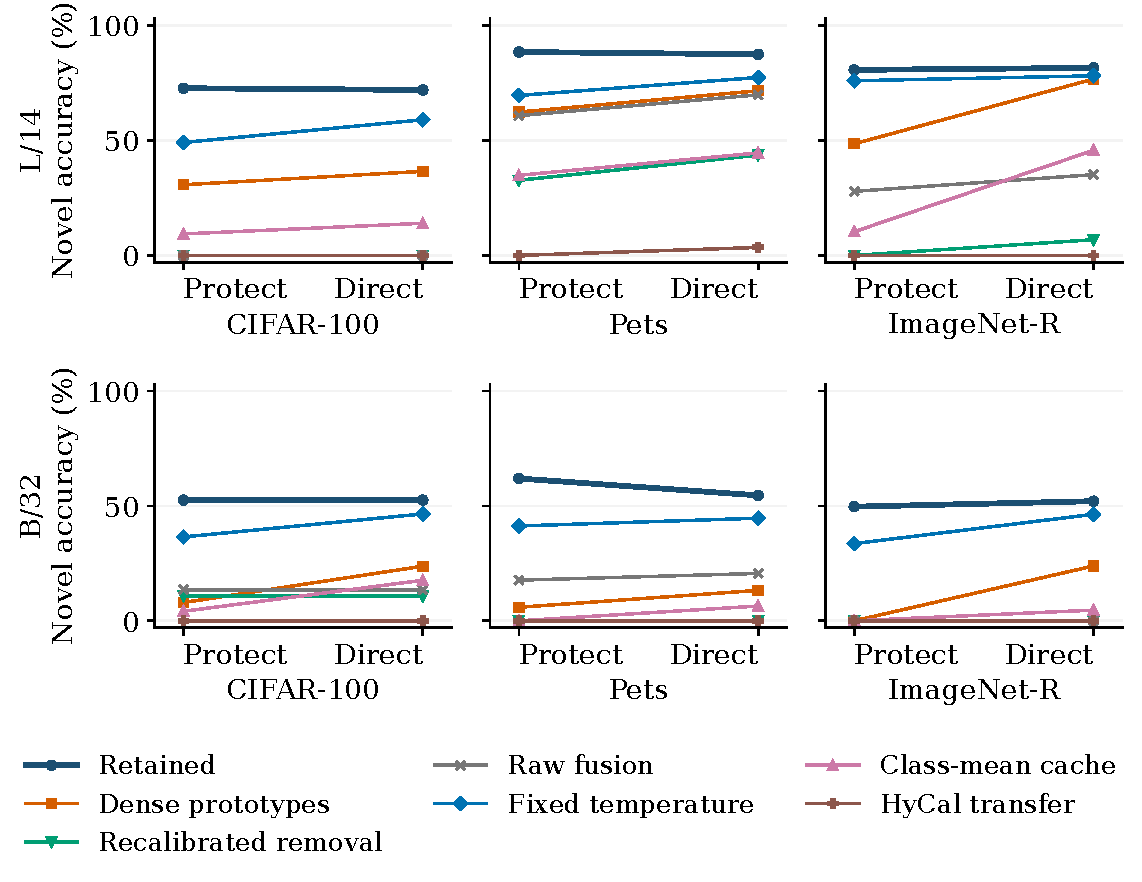
\includegraphics[width=.98\textwidth]{calibration_fairness.pdf}
\caption{Calibration-rule comparison at identical cap-40 coverage, fifth arrival, first prespecified order. Lines connect the sufficient protection test and the direct paired accuracy test for each readout. Novel means cover all ten partitions, with zero for reference fallback. Each test uses 95\% retention and 95\% confidence over five prespecified arrivals within a fixed configuration. Admission counts, conditional accuracy and empirical target attainment are reported in Supplementary Section N.}
\label{fig:fairness}
\end{figure}

\clearpage
\begin{table}[H]
\centering
\setlength{\belowcaptionskip}{8pt}
\caption{Protection-risk-calibrated admission after the fifth arrival in the first prespecified order, with up to 40 images per base class, 95\% retention and 95\% five-session confidence. Queries are actual base-calibration counts; Finite counts certified expansion and Test met counts attained test targets. Base/Novel are test percentages, mean $\pm$ sample standard deviation over ten partitions, including fallback. All six readouts are reported in Supplementary Section L.}
\label{tab:riskmain}
{\small\setlength{\tabcolsep}{4pt}\begin{tabular}{@{}lrrrrr@{}}
\toprule
Dataset & Calibration & \multicolumn{2}{c}{Admission} & \multicolumn{2}{c}{Test accuracy (\%) $\uparrow$} \\
\cmidrule(lr){3-4}\cmidrule(l){5-6}
& Queries & Finite & Test met & Base & Novel \\
\midrule
\multicolumn{6}{@{}l}{\textit{CLIP ViT-L/14}} \\
CIFAR-100 & 1600 & 10/10 & 10/10 & 85.86\,\ensuremath{\pm}\,1.19 & 72.76\,\ensuremath{\pm}\,4.76 \\
Pets & 600 & 10/10 & 10/10 & 94.10\,\ensuremath{\pm}\,2.27 & 88.51\,\ensuremath{\pm}\,4.85 \\
ImageNet-R & 3636--3778 & 10/10 & 10/10 & 89.02\,\ensuremath{\pm}\,0.51 & 80.74\,\ensuremath{\pm}\,1.83 \\
\midrule
\multicolumn{6}{@{}l}{\textit{CLIP ViT-B/32}} \\
CIFAR-100 & 1600 & 10/10 & 10/10 & 76.74\,\ensuremath{\pm}\,1.73 & 52.54\,\ensuremath{\pm}\,4.34 \\
Pets & 600 & 10/10 & 10/10 & 88.10\,\ensuremath{\pm}\,3.41 & 61.94\,\ensuremath{\pm}\,14.07 \\
ImageNet-R & 3636--3778 & 10/10 & 10/10 & 72.98\,\ensuremath{\pm}\,1.21 & 49.67\,\ensuremath{\pm}\,2.38 \\
\bottomrule
\end{tabular}
}
\end{table}

At cap 40, retained tables certify final-session expansion in all ten partitions of each dataset and encoder, with all test targets met (Table~\ref{tab:riskmain}). L/14 novel accuracy is 72.76\% on CIFAR, 88.51\% on Pets and 80.74\% on ImageNet-R. All 20 arrival paths per dataset/encoder meet every test target. Finite admission holds throughout all CIFAR and ImageNet-R paths and 17/20 L/14 and 16/20 B/32 Pets paths; the remaining Pets paths use an early-session fallback. Full comparisons distinguish policy gains, which include fallback, from accuracy differences on jointly admitted partitions. The common protection criterion remains conservative for replacement models that recover reference errors.

\subsection{Separating recognition from certification}
Figure~\ref{fig:fairness} holds calibration images, candidate thresholds and error allocation fixed while changing the statistical criterion. On ImageNet-R L/14, crediting recovered errors raises dense-prototype admission from 9/10 to 10/10 and fallback-inclusive novel accuracy from 48.58\% to 76.76\%. Retained tables attain 81.61\%, a paired gain of 4.85 [2.78,6.93] points on ten jointly admitted partitions.

Table~\ref{tab:policycapacity} separates selected-policy gains from recognition capacity on the same fitted models. At the shared 95\% minimum target, retained-minus-dense capacity gains are 3.68 [1.08,6.38] points on CIFAR L/14 and 10.40 [7.31,14.64] on ImageNet-R B/32, with ten and nine jointly feasible partitions. L/14 ImageNet-R capacities of 83.93\% and 83.64\% yield a 0.29 [$-0.55$,1.16]-point difference, while Pets L/14 favors dense prototypes by 2.12 points. Retained readouts therefore supply their clearest common-target capacity gains on CIFAR L/14 and ImageNet-R B/32; policy selection contributes separately to the realized differences.

\begin{table}[!htbp]
\centering\setlength{\belowcaptionskip}{8pt}
\caption{Retained-minus-dense selected-policy and descriptive capacity gains (pp), fifth arrival, first order. Capacity uses the common 95\% minimum base target. Within a row, both columns use the same jointly feasible partitions (count); policy means include reference fallback. Brackets give conditional paired 95\% bootstrap intervals on fixed images.}
\label{tab:policycapacity}
{\small\setlength{\tabcolsep}{3pt}\resizebox{\linewidth}{!}{\begin{tabular}{@{}llrrr@{}}
\toprule
Encoder & Data & Policy gap & Common-floor capacity gap & Matched count \\
\midrule
L/14 & CIFAR-100 & +35.40 [+16.61,+54.61] & +3.68 [+1.08,+6.38] & 10/10 \\
L/14 & Pets & +15.88 [-1.27,+40.52] & -2.12 [-4.07,-0.49] & 10/10 \\
L/14 & ImageNet-R & +4.85 [+2.77,+6.93] & +0.29 [-0.55,+1.16] & 10/10 \\
B/32 & CIFAR-100 & +26.38 [+11.60,+41.41] & +3.50 [-0.47,+7.94] & 9/10 \\
B/32 & Pets & +42.92 [+15.13,+66.79] & +1.17 [-5.91,+7.38] & 8/10 \\
B/32 & ImageNet-R & +26.15 [+15.85,+37.54] & +10.40 [+7.31,+14.64] & 9/10 \\
\bottomrule
\end{tabular}
}}
\end{table}

At the dense policy's actual, stricter base accuracy, conservative alignment on ImageNet-R L/14 yields a 3.23 [1.48,5.02]-point retained-minus-selected-dense gain, with mean base overshoot 0.027 points. Comparing both frontiers at that target yields 3.10 [1.37,4.88] points. These target-specific comparisons distinguish recognition capacity from threshold-selection effects. Section P supplies exact discrete matching and all conditions. Section N reports both prespecified calibration policies, admission counts, conditional accuracy and fallback-inclusive results, including 9/10 direct-calibrated retained admissions on B/32 Pets and one dense B/32 ImageNet-R test-target miss.

Query centering has an exact interpretation as a query-dependent admission offset,
$d_{\mathrm{eff}}(x)=d+a\mu_L(x)/\sigma_L(x)-u\mu_P(x)/\sigma_P(x)$,
after removing text shifts common to all candidates. Its contribution operates through the combined decision margin: adding it improves group-ranking AUROC by .054 and .048 on ImageNet-R with L/14 and B/32. The offset term alone has novel-positive AUROC below .5 in all six conditions (Section P).

\subsection{Calibration under query distribution shift}
\label{sec:shift}
The controlled CIFAR stress test uses clean fitting/support and noisy or blurred queries. Clean calibration meets 5/10 and 1/10 L/14 final targets; matching calibration restores 10/10 with finite admission for both encoders (Section O).

We additionally transfer the frozen ImageNet-R readouts to matching ImageNet-Sketch classes~\cite{wang2019robustglobal}. Before target scoring, identity checks remove source overlaps and target duplicates, retaining 6,445 images: 2,492 for calibration and 3,953 for test. Source and Sketch calibration use equal per-class counts; model parameters and source support remain fixed. With direct Sketch calibration, retained readouts reach 86.82\% and 58.96\% novel accuracy with L/14 and B/32, respectively, with finite admission and target attainment in all ten partitions. Source calibration also meets these targets, at 82.99\% and 54.87\% novel accuracy. At the common 95\% minimum target, L/14 retained and dense capacities both round to 88.84\%; B/32 retention supplies a 5.78 [4.03,7.55]-point capacity gain on nine jointly feasible partitions. Section R reports the identity exclusions, absolute base accuracies, both calibration criteria and exact frontiers.

\section{Conclusion}
Candidate tables connect retained discrimination to retention-constrained expansion. Fixed base references preserve the score frame, query-dependent normalization aligns heterogeneous evidence, and independent calibration selects novel admission. Equal-budget fusion comparisons identify a normalization benefit on ImageNet-R with both encoders; matched frontiers locate the classifier's contribution at specific operating targets. Frozen-model Sketch validation demonstrates useful admission on identity-disjoint natural-shift images. These results provide a practical way to measure and control how an existing classifier supports an expanding label vocabulary.

\section*{CRediT authorship contribution statement}
Junyi Zhang: Conceptualization, Methodology, Software, Validation, Formal analysis, Investigation, Data curation, Visualization, Writing -- original draft, Writing -- review and editing.

\section*{Funding}
This research did not receive any specific grant from funding agencies in the public, commercial, or not-for-profit sectors.

\section*{Declaration of competing interest}
The author declares that there are no known competing financial interests or personal relationships that could have appeared to influence the work reported in this paper.

\section*{Data availability}
The experiments use public CIFAR-100, Oxford-IIIT Pets, ImageNet-R and ImageNet-Sketch data and the publicly released CLIP ViT-L/14 and ViT-B/32 checkpoints. Code, source-hashed experimental records, prediction archives, manuscript sources, and table/figure generation scripts are available at \url{https://github.com/Cheerssom/Reference-Anchored-Candidate-Tables}. Dataset images, pretrained weights, and feature caches are obtained separately using the repository instructions.

\section*{Declaration of generative AI and AI-assisted technologies in the manuscript preparation process}
OpenAI Codex was used to assist with literature discovery, manuscript drafting and revision, experiment and verification scripts, and LaTeX and table preparation. The author is responsible for the accuracy, interpretation and originality of the submitted work and for reviewing and approving the final manuscript and supporting materials.

\bibliographystyle{elsarticle-num}
\bibliography{references}
\end{document}
